\documentclass[border=6pt]{standalone}
\usepackage{tikz}
\begin{document}
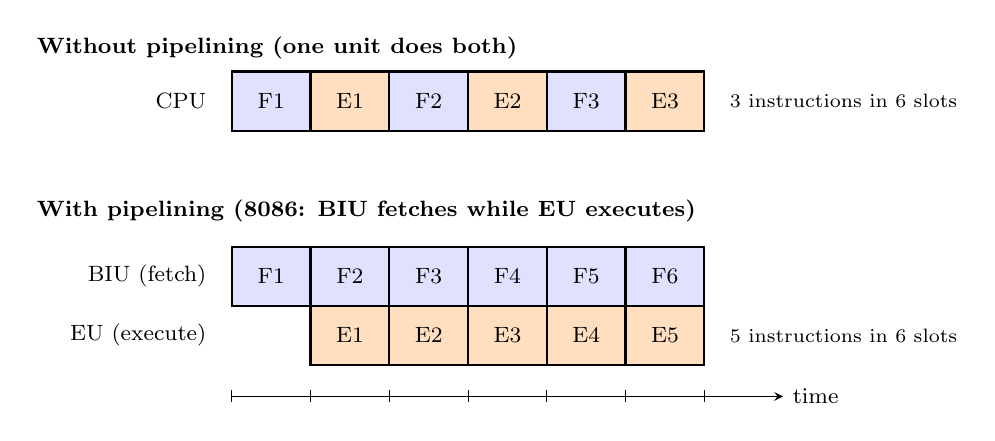
\begin{tikzpicture}[font=\small,x=1.0cm,y=0.75cm,
 F/.style={draw,thick,fill=blue!12,minimum width=1cm,minimum height=0.75cm,inner sep=0,font=\footnotesize},
 E/.style={draw,thick,fill=orange!25,minimum width=1cm,minimum height=0.75cm,inner sep=0,font=\footnotesize}]
\node[font=\footnotesize\bfseries,anchor=west] at (-2.6,0.9) {Without pipelining (one unit does both)};
\foreach \i/\x in {1/0,2/2,3/4} { \node[F] at (\x+0.5,0) {F\i}; \node[E] at (\x+1.5,0) {E\i}; }
\node[anchor=east,font=\footnotesize] at (-0.2,0) {CPU};
\node[font=\scriptsize,anchor=west] at (6.2,0) {3 instructions in 6 slots};
\begin{scope}[yshift=-2.6cm]
\node[font=\footnotesize\bfseries,anchor=west] at (-2.6,1.6) {With pipelining (8086: BIU fetches while EU executes)};
\node[anchor=east,font=\footnotesize] at (-0.2,0.5) {BIU (fetch)};
\node[anchor=east,font=\footnotesize] at (-0.2,-0.5) {EU (execute)};
\foreach \i in {1,...,6} \node[F] at (\i-0.5,0.5) {F\i};
\foreach \i in {1,...,5} \node[E] at (\i+0.5,-0.5) {E\i};
\node[font=\scriptsize,anchor=west] at (6.2,-0.5) {5 instructions in 6 slots};
\end{scope}
\draw[->,>=stealth] (0,-5.0) -- (7.0,-5.0) node[right,font=\footnotesize]{time};
\foreach \t in {0,...,6} \draw (\t,-4.9) -- (\t,-5.1);
\end{tikzpicture}
\end{document}
